\chapter{Results}\label{ch:results}

This chapter presents the experimental results of different DIP-based denoising approaches.
We first evaluate these methods on standard image datasets, providing a controlled setting for method comparison.
Then, we apply these approaches to DAS data demonstrating its performance in a more complex real-world scenario.

\section{Image Data}

Since clean reference samples are not available for DAS data, we begin by conducting experiments on standard image denoising tasks.
These preliminary evaluations enable a controlled comparison of different methods and configurations.

For all variants, we follow the original DIP paper and set the maximum number of iterations to 2000.
For ES-based methods, we employ the ES-WMV criterion with a patience of 500 iterations.
For DIP-TV, we set $\lambda = 0.1$, and for SG-DIP, we set the number of different noise samples per iteration to 3, as recommended in the original paper.
For SGR-DIP, we linearly increase $\lambda$ from 1 to 10 throughout training. 
As discussed in Section~\ref{sec:architecture}, we use ECA in the skip connections because it tends to retain more fine-grained details, while yielding almost identical performance, as shown in Table~\ref{tab:ECA}. 

\begin{table}
    \small
    \centering
    \begin{tabular}{ l l c c }
        \toprule
        Skip Type &Method &PSNR (dB) $\uparrow$ &SSIM $\in [0,1]$ $\uparrow$ \\
        \midrule
        \multirow{2}{4em}{Conv} &SG-DIP (ES) &26.03 {\scriptsize (2.15)} &0.68 {\scriptsize (0.11)} \\
        &SGR-DIP &\underline{26.34} {\scriptsize (2.12)} &\textbf{0.70} {\scriptsize (0.11)} \\
        \midrule
        \multirow{2}{4em}{ECA} &SG-DIP (ES) &25.97 {\scriptsize (1.92)} &0.68 {\scriptsize (0.11)} \\
        &SGR-DIP &\textbf{26.37} {\scriptsize (2.04)} &\textbf{0.70} {\scriptsize (0.11)} \\
        \bottomrule
    \end{tabular}
    \caption{
        Comparison of different types of skip connections on the Set14 dataset.
        Noisy input images are generated at a PSNR of 15\,dB.
        Values represent mean and {\scriptsize (standard deviation)}.
    }\label{tab:ECA}
\end{table}

We conduct a series of experiments to evaluate the performance of different approaches.

First, we compare the methods on the Set14 dataset at both low and high noise levels.
At low noise levels, all variants --- except for DDIP --- achieve satisfactory results.
However, at high noise levels, explicit regularization becomes crucial, as overfitting occurs very early in the optimization process (see Figure~\ref{fig:noise-levels}).
Among the tested methods, only the ES-based methods and our SGR-DIP are robust across different noise levels, with DIP-TV with ES being the most consistent (see Table~\ref{tab:noise-levels}).

We further evaluate the variants on the CBSD68 dataset with moderate noise added.
While our approach yields the best results, it takes significantly longer to run compared to other methods.
The best tradeoff between denoising performance and runtime is achieved by DIP-TV with ES, as shown in Table~\ref{tab:CBSD68}.
However, in terms of visual quality, it is clearly outperformed by our SGR-DIP, as demonstrated in Figure~\ref{fig:CBSD68}.

\begin{table}
    \small
    \centering
    \begin{tabular}{ l c c c c }
        \toprule
        &\multicolumn{2}{c}{20\,dB} &\multicolumn{2}{c}{10\,dB}\\
        \midrule
        Method &PSNR (dB) $\uparrow$ &SSIM $\in [0,1]$ $\uparrow$ &PSNR (dB) $\uparrow$ &SSIM $\in [0,1]$ $\uparrow$\\
        \midrule
        DIP &27.52 {\scriptsize (1.20)} &0.74 {\scriptsize (0.04)} &16.02 {\scriptsize (0.45)} &0.21 {\scriptsize (0.06)} \\
        DIP (ES) &27.10 {\scriptsize (1.72)} &0.73 {\scriptsize (0.09)} &22.52 {\scriptsize (1.58)} &0.48 {\scriptsize (0.05)} \\
        DIP-TV &28.29 {\scriptsize (2.31)} &\textbf{0.79} {\scriptsize (0.06)} &18.99 {\scriptsize (0.52)} &0.33 {\scriptsize (0.07)} \\
        DIP-TV (ES) &\underline{28.37} {\scriptsize (2.31)} &0.78 {\scriptsize (0.06)} &\underline{23.44} {\scriptsize (1.67)} &\textbf{0.56} {\scriptsize (0.08)} \\
        DDIP &23.15 {\scriptsize (2.84)} &0.58 {\scriptsize (0.14)} &22.58 {\scriptsize (2.57)} &0.54 {\scriptsize (0.10)} \\
        SG-DIP &\textbf{28.50} {\scriptsize (1.97)} &\textbf{0.79} {\scriptsize (0.07)} &12.34 {\scriptsize (1.16)} &0.12 {\scriptsize (0.05)} \\
        SG-DIP (ES) &27.42 {\scriptsize (2.40)} &0.75 {\scriptsize (0.09)} &\textbf{23.49} {\scriptsize (2.16)} &0.54 {\scriptsize (0.10)} \\
        SGR-DIP &26.99 {\scriptsize (2.36)} &0.73 {\scriptsize (0.13)} &23.29 {\scriptsize (2.48)} &\textbf{0.56} {\scriptsize (0.12)} \\
        \bottomrule
    \end{tabular}
    \caption{
        Quantitative comparison of DIP variants on the Set14 dataset at different noise levels.
        Noisy input images are generated at PSNRs of 20\,dB and 10\,dB, respectively.
        Values represent mean and {\scriptsize (standard deviation)}.
    }\label{tab:noise-levels}
\end{table}

\begin{figure}
    \centering
    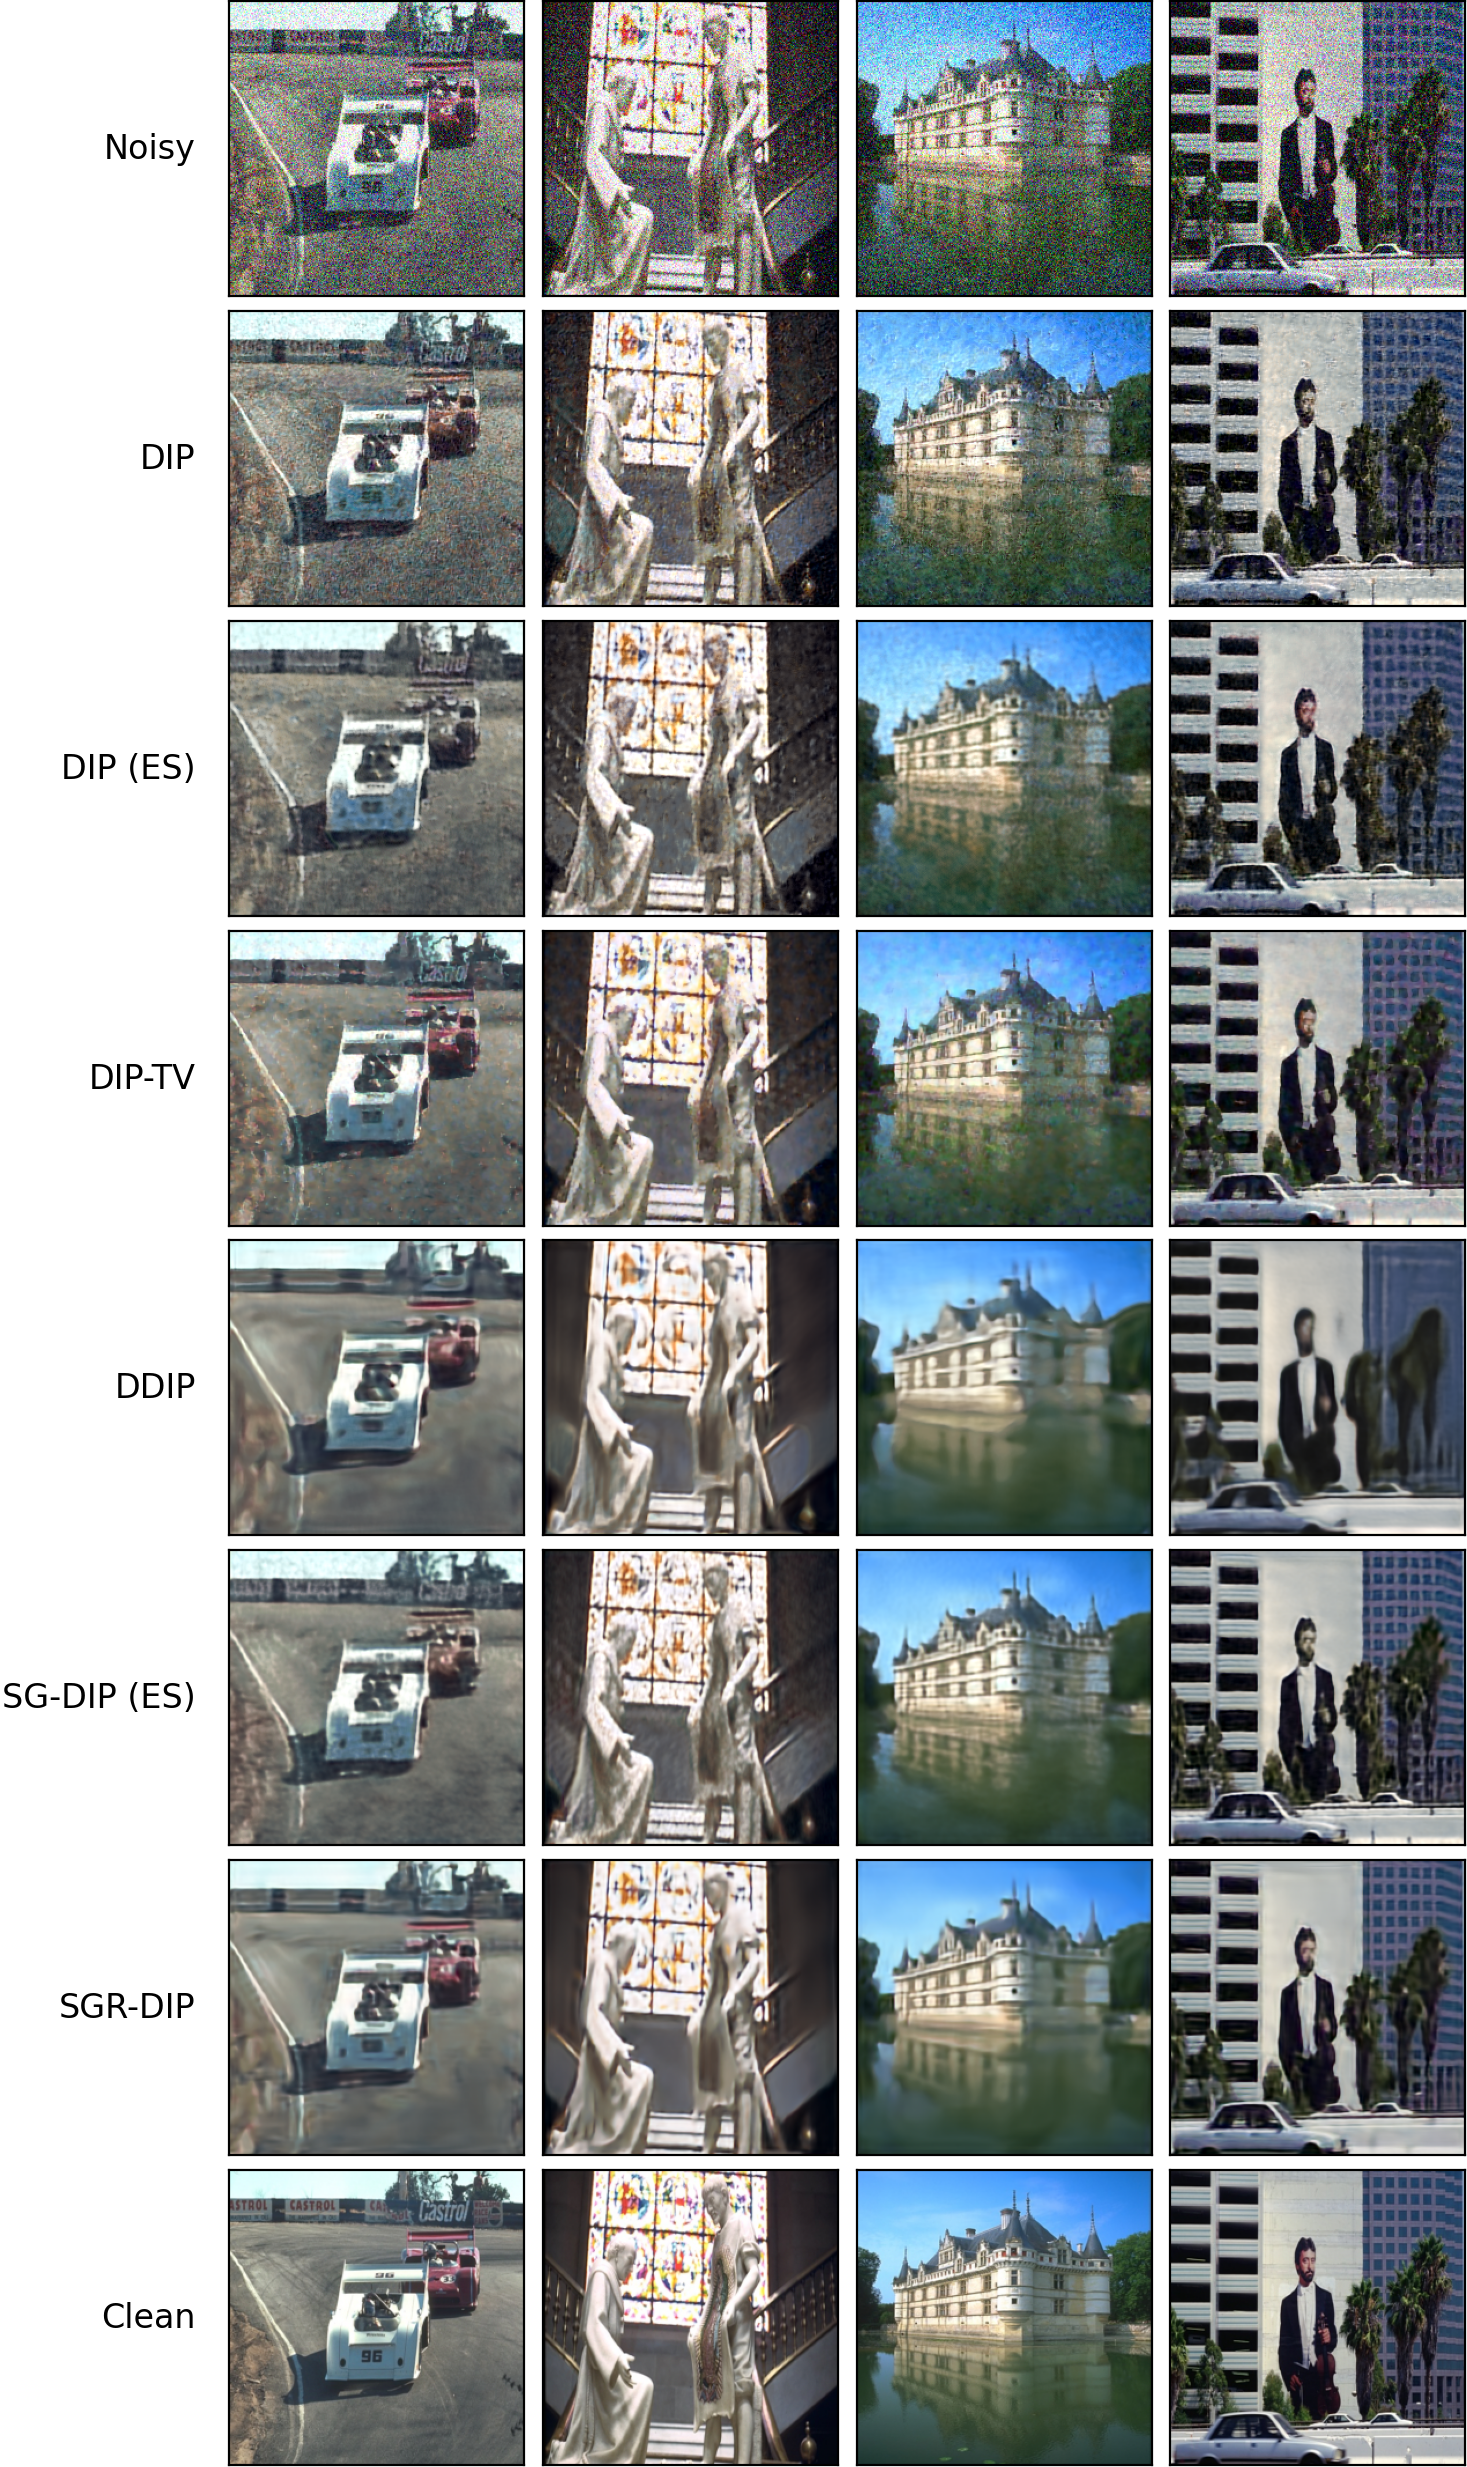
\includegraphics[width=\textwidth]{img/fig_6.1.png}
    \caption{
        Mean PSNR curves of DIP variants on the Set14 dataset at different noise levels.
        Noisy input images are generated at PSNRs of 20\,dB and 10\,dB, respectively.
        Dashed lines represent the average detected stopping points for the corresponding ES-based methods.
    }\label{fig:noise-levels}
\end{figure}

\begin{table}
    \small
    \centering
    \begin{tabular}{ l c c c }
        \toprule
        Method &PSNR (dB) $\uparrow$ &SSIM $\in [0,1]$ $\uparrow$ &Runtime (m) $\downarrow$\\
        \midrule
        DIP &22.32 {\scriptsize (0.74)} &0.43 {\scriptsize (0.11)} &1.31 {\scriptsize (0.01)} \\
        DIP (ES) &25.64 {\scriptsize (2.07)} &0.62 {\scriptsize (0.07)} &\textbf{0.50} {\scriptsize (0.08)} \\
        DIP-TV &26.06 {\scriptsize (1.37)} &0.65 {\scriptsize (0.07)} &1.45 {\scriptsize (0.01)} \\
        DIP-TV (ES) &\underline{26.65} {\scriptsize (2.45)} &\underline{0.69} {\scriptsize (0.10)} &\underline{0.67} {\scriptsize (0.16)} \\
        DDIP &24.54 {\scriptsize (3.15)} &0.61 {\scriptsize (0.13)} &1.34 {\scriptsize (0.01)} \\
        SG-DIP &22.24 {\scriptsize (3.88)} &0.45 {\scriptsize (0.09)} &3.33 {\scriptsize (0.02)} \\
        SG-DIP (ES) &26.57 {\scriptsize (2.47)} &\underline{0.69} {\scriptsize (0.09)} &2.05 {\scriptsize (0.61)} \\
        SGR-DIP &\textbf{26.76} {\scriptsize (2.51)} &\textbf{0.70} {\scriptsize (0.10)} &3.34 {\scriptsize (0.09)} \\
        \bottomrule
    \end{tabular}
    \caption{
        Quantitative comparison of DIP variants on the CBSD68 dataset.
        Noisy input images are generated at a PSNR of 15\,dB.
        Values represent mean and {\scriptsize (standard deviation)}.
    }\label{tab:CBSD68}
\end{table}

\begin{figure}
    \centering
    \includegraphics[width=\textwidth]{img/fig_6.2_1.png}\\
    \vspace{20pt}
    \includegraphics[width=\textwidth]{img/fig_6.2_2.png}
    \caption{
        Visual comparison of DIP variants on the CBSD68 dataset.
        Noisy input images are generated at a PSNR of 15\,dB.
    }\label{fig:CBSD68}
\end{figure}

\section{Distributed Acoustic Sensing Data}
